\section{Models}

RDBMS are for small scale applications running on a single machine. We can either scale up (costly) or scale out (complex, high maintenance cost).



\subsection{Wide Column Stores}

Wide column stores are a type of NoSQL DB. Also uses tables, rows and columns but the names and the format of the columns can vary from row to row in the same table. Interpret this as a two-dimensional key-value store. In WCS, we store together what is accessed together - good for distributed systems since it reduces the amount of data transferred.

\begin{figure}[h]
	\centering
	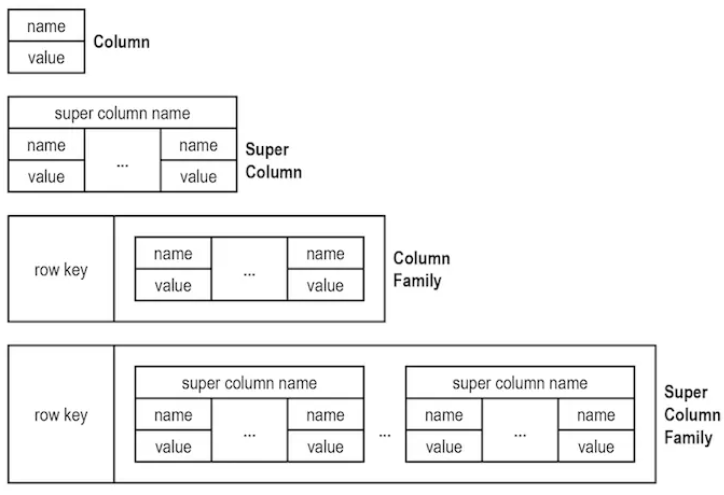
\includegraphics[scale=0.6]{images/3-terminology.PNG}
	\caption{WCS DB objects.}
	\label{fig:term}
\end{figure}

Column families have to be specified in advance, but columns can be added on the fly (see Figure \ref{fig:wcs_ex}). The row ID is always its own column. %TODO right?

\begin{figure}[h]
	\centering
	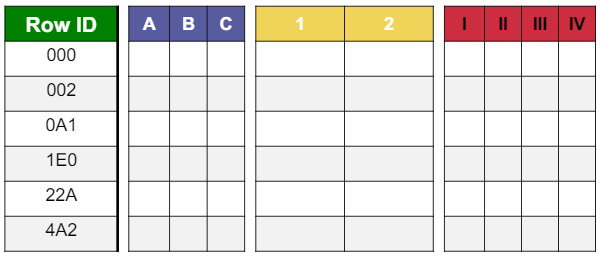
\includegraphics[scale=0.6]{images/3-wcs_ex.PNG}
	\caption{WCS example - individual columns can be added on the fly.}
	\label{fig:wcs_ex}
\end{figure}

\paragraph{Usual Column Store}
CS columnar data layout is adopted s.t. each column is stored separately on disk. In WCS, column families containing multiple columns are stored together in a row-by-row fashion by column family.


\subsubsection{Bigtable}

See reading assignment "Bigtable: A Distributed Storage System for Structured Data". The following is a brief summary of this paper.

\paragraph{Introduction}
\begin{itemize}
    \item \textbf{Bigtable is a distributed storage system for managing structured data that is designed to scale to a very large size (PB across thousands of servers).}
    \item Build on top of GFS (similar to HDFS).
    \item Serves applications with varying demands (data size and latency). Throughput-oriented batch processing vs. latency-sensitive jobs serving data to real-time users.
    \item Clients have dynamic control over data layout and format (locality).
    \item Wide applicability, scalability, high performance, high availability.
    \item No support for a full relational model.
    \item Data is indexed using row and column names (arbitrary strings). Data is treated as uninterpreted strings (clients serialize structured / semi-structured data into these strings).
    \item Data can be served out of memory or disk (client decision).
\end{itemize}

\paragraph{Data Model}
Sparse, distributed, persistent multi-dimensional sorted map. Example in Figure \ref{fig:bt_ex}.

(row:string, column:string, time:int64) $\longrightarrow$ string

\begin{figure}[h]
	\centering
	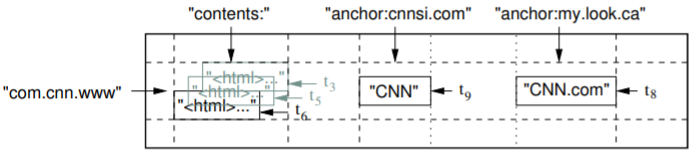
\includegraphics[scale=0.6]{images/3-bt_ex.PNG}
	\caption{Bigtable Web pages example.}
	\label{fig:bt_ex}
\end{figure}

\textbf{Rows:} Row keys are arbitrary strings (up to 64KB, usually sub 100B). Read/write under single row key is atomic. Sorted in lexicographical order. Table row range is dynamically partitioned (horizontally) into \textbf{tablets} (unit of distribution and load balancing).

\textbf{Column Families:} Column keys are grouped into column families = basic unit of access control and disk/memory accounting. Data in CF usually of same type. Families created in advance - small number, individual cols unbounded number. Column key: \textit{family:qualifier} (qualifier can be empty if family contains only one col).

\textbf{Timestamps:} Cells can contain multiple versions of same data indexed by a 64b timestamp. For applications wanting to avoid collisions, timestamps have to be unique. Most recent version is read first. Client specifies: either keep only last $n$ values or only new-enough values.

\paragraph{API}
\begin{itemize}
    \item Create and delete tables and col. families.
    \item Changing cluster, table and col. family metadata (e.g. access control rights).
    \item Write, delete values. Look up values from individual rows or iterate over subset of data.
    \item Iterate over multiple col. families, possible to limit rows, cols, timestamps produced by a scan.
    \item Single-row transactions to perform atomic read-modify-write sequences (single row key).
    \item No transactions over several row keys but writes across row keys can be batched.
    \item Cells can be used as integer counters.
    \item Client-supplied scripts can be executed in address space of servers (Sawzall language).
    \item MapReduce can be used.
\end{itemize}

\paragraph{Building Blocks}
\begin{itemize}
    \item On top of GFS - stores log and data files.
    \item Bigtable depends on cluster management system for scheduling jobs, managing resources on shared machines, dealing with machine failures and monitoring machine status.
    \item Store any Bigtable data: \textbf{SSTable} file format used internally = persistent and ordered immutable map from keys to values (arbitrary byte strings).
    \item Point queries and range queries are possible (key-value operations).
    \item SSTable divided into sequence of GFS blocks. At end of SSTable - block index keeping track of GFS block locations.
    \item Opening SSTable - block index is loaded into memory.
    \item Lookup: single disk seek (binary search on in-memory index and read appropriate block from disk).
    \item Optionally: completely map SSTable into memory (no disk seeks).
    \item Bigtable relies on highly avaliable and persistend distributed lock service \textbf{Chubby}. Why: store bootstrap location of Bigtable data, discover tablet servers, finalize tablet server deaths, store schema info (col. family info for each table), store access control lists.
\end{itemize}

\textbf{Chubby Service:} Five active replicas (Paxos for consistency), one is master service and serves requests. Namespace with directories and small files, both of with can be used as locks. Atomic reads and writes to files.

\textbf{Chubby Client:} Consistent caching of Chubby files. Clients maintain session with service (needs to be renewed continuously, else client loses locks).


\paragraph{Implementation}
Library linked into every client, one master server, many tablet servers (dynamic add / remove possible).
\begin{itemize}
    \item \textbf{Master Server:} Assigning tablets to tablet servers, detect addition / expiration of tablet servers, balancing load, garbage collection of GFS files, handle schema changes (table / col. family deletion / creation).
    \item \textbf{Tablet Server:} Manages set of tablets, handle read / write requests, splits too large tablets.
    \item \textbf{Client Communication:} Not through master! Communicaton directly to tablet servers (read / write). Client does not have to ask master for tablet location information.
\end{itemize}

\paragraph{Tablet Location}
Three level hierarchy to store tablet location information in memory (see Figure \ref{fig:bt_loc}). Chubby file contains location of root tablet. Root tablet (never split) contains location of all tablets in special METADATA table. Each METADATA tablet contains location of a set of user tablets (row key = encoding of tablet's table ID and end row).

Client can cache tablet locations (GFS accesses not required). Clients also prefetch table locations.

METADATA also stored log of all events pertaining to each tablet for debugging and performance analysis.

\begin{figure}[h]
	\centering
	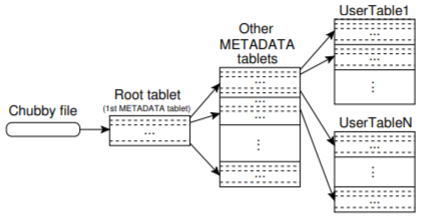
\includegraphics[scale=0.7]{images/3-bt_location.PNG}
	\caption{Tablet location hierarchy.}
	\label{fig:bt_loc}
\end{figure}

\paragraph{Tablet Assignment}
Each tablet assigned to one tablet server at a time. Master keeps track of live TS and current assignments (and unassigned tablets). Unassigned tablets are assigned to TS with enough room by master.

Chubby keeps track of tablet servers. On startup, TS receive x-lock on unique file in Chubby directory (monitored by master to discover TS).

Master reassigns tablets from dead TS into unassigned pile. Monitor TS with periodic check of lock status. Current assignments don't change if master fails.

(More details are omitted here).

\paragraph{Tablet Serving}
Persistent state of a tablet stored in GFS. Updates are committed to a commit log storing redo records. (Recovery details omitted).

Write: TS checks well-formedness and user authorization. If valid, write to commit log stored in GFS (disk). Write contents stored in memtable (RAM).

Read: TS checks well-formedness and user authorization. If valid, execute read on merged view of sequence of SSTables and memtable (disk and RAM). Merge easy since both are lexicographically sorted.

\paragraph{Compactions}
\begin{itemize}
    \item Minor compaction: if memtable to big, write to GFS as SSTable and create new memtable.
    \item Merging compaction: periodically executed to merge sequence of SSTables and memtable (in background) into a new SSTable.
    \item Major compaction: rewrite all SSTables into one - contains no deleted values.
\end{itemize}


\paragraph{Refinements}
\begin{itemize}
    \item \textbf{Locality Group:} Client group multiple col. families together into separate SSTable for efficient reads. Locality groups can be declared to be in RAM (lazy loading). Useful for small pieces of data accessed frequently. E.g. used for METADATA table.
    \item \textbf{Compression:} Client can choose if and how LG on SSTable is compressed - applied to each SSTable block (don't need to decompress whole table for small read).
    \item \textbf{Caching:} Speed up reads with two layer caching at TS. One for frequent and one for locality.
    \item \textbf{Bloom Filters:} Reduce number of disk accessed on a read (SSTables) by using BF in SSTables for specific LG (chosen by client). If SSTable might contain data we want, it is fetched.
    \item \textbf{Commit Log:} ommitted.
    \item \textbf{Tablet Recovery:} ommitted.
    \item \textbf{Exploit Immutability:} ommitted.
\end{itemize}

\paragraph{Performance Evaluation}
Ommitted.

\paragraph{Lessons Learned}
Ommitted.

\paragraph{Related Work}
Ommitted.


%TODO Webtable example more? also used by HBase


\subsubsection{HBase}

See reading assignment "HBase: The Definitive Guide". The following is a brief summary of chapters 1, 3 and 8. Some things are also from chapter 20 of "Hadoop: The Definitive Guide".

\paragraph{Basics}
\begin{itemize}
    \item \textbf{HBase is a distributed column-oriented database built on top of HDFS. Used when real-time read/write random access on very large datasets is required.}
    \item HBase scales linearly just by adding nodes.
    \item Not relational, no support for SQL.
    \item Hosts very large, sparsely populated tables on clusters made from commodity hardware.
    \item \textbf{Data Model:} Applications store data in labeled tables. Tables are made of rows and columns. Table rows are sorted by row key (primary key, byte arrays) - byte-ordered. Table cells — the intersection of row and column coordinates — are versioned. By default, their version is a timestamp auto-assigned by HBase at the time of cell insertion. A cell’s content is an uninterpreted array of bytes (same as Bigtable). See example in Figure \ref{fig:hb_ex}.
    \item Physically, column families are stored together on HDFS. Members should have same characteristics and access pattern.
    \item \textbf{Regions:} Tables automatically partitioned horizontally into regions (same as tablets in Bigtable). First row inclusive, last row exclusive.
    \item \textbf{Locking:} Row updates are atomic.
    \item Same physical layout as HDFS with different words (see Figure \ref{fig:hb_phys}).
    \item HMaster responsible for bootstrapping, assigning regions to registered regionservers and for recovering regionserver failures. Regionservers serve client read/write requests and manage region splits.
\end{itemize}

%TODO ZooKeeper?

\begin{figure}[h]
	\centering
	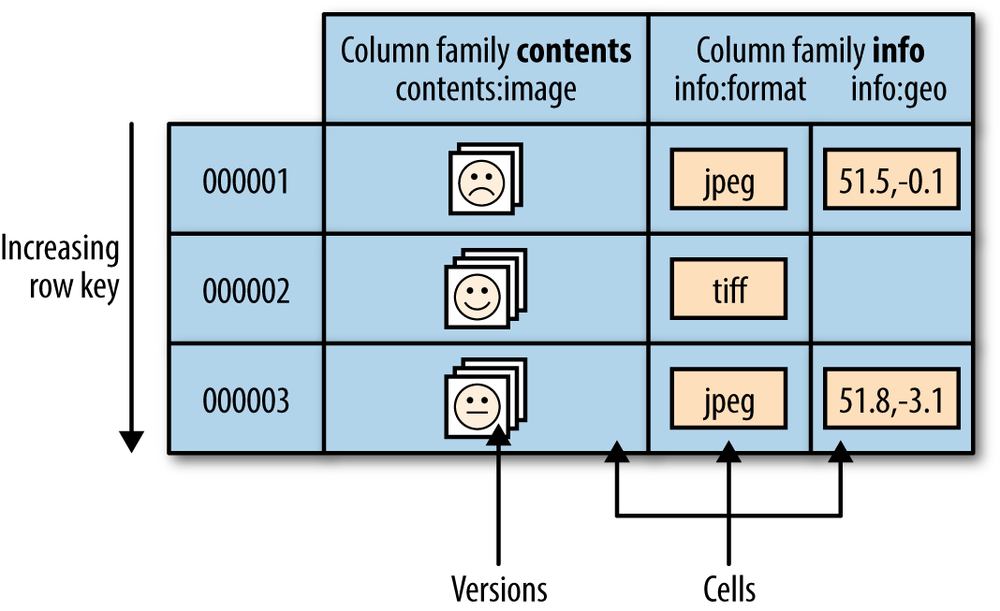
\includegraphics[scale=0.3]{images/3-hbase.png}
	\caption{HBase data model example.}
	\label{fig:hb_ex}
\end{figure}

\begin{figure}[h]
	\centering
	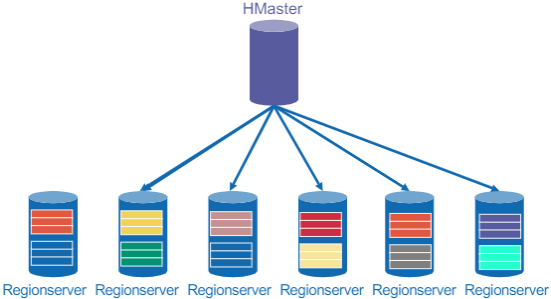
\includegraphics[scale=0.7]{images/3-hb_phys.PNG}
	\caption{HBase implementation model.}
	\label{fig:hb_phys}
\end{figure}

%TODO HBase definitive guide reading, VIS summary
















%HBase (on top of HDFS) - logical and physical model

%hbase stores data in a structured way vs. just drop your files and let upper layers handle it - ETL approach (structured) (prepopulated DB vs querying simple files on top of storage layer)


%TODO log structured merge trees - maybe memtable thing with more detail again

\url{http://www.benstopford.com/2015/02/14/log-structured-merge-trees/}

%TODO HFile compaction - short circuit (locality)





\subsection{Data Models and Schemas}

Physical view: actual syntax (CSV, JSON, XML, etc.). Logical view: data model (e.g. relational table). A physical view can be interpreted with different logical views. E.g. relational table, Excel spreadsheet, etc.

\paragraph{Structured Data}
Data that is easy to search and organize, usually contained in rows and columns with its elements mapped into fixed pre-defined fields. Often managed by SQL.

\paragraph{Unstructured Data}
Data that cannot be contained in a row-column database and that doesn't have an associated data model. Difficult to search, manage and analyse. Usually accessed and processed with ML / AI technologies. E.g. text.

\paragraph{Semi-Structured Data}
Mix of the two above. Data with defining / consistent characteristics but not conforming to rigid structures - usually just data where heterogeneity and nestedness is allowed. Usually comes with metadata to make it easier to organize. E.g. Email messages (text unstructured but everything else structured.


\subsubsection{JSON Data Model}

JSON documents can be interpreted as trees (see Figure \ref{fig:jsontree}). In JSON, labels are on the edges (in contrast to XML where labels are in nodes).

\begin{figure}[h]
	\centering
	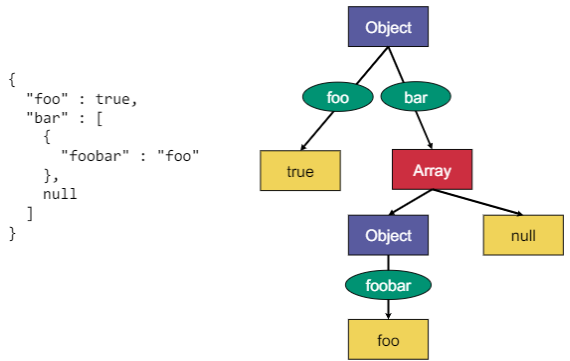
\includegraphics[scale=0.7]{images/3-jsontree.PNG}
	\caption{Tree-based visual model of JSON.}
	\label{fig:jsontree}
\end{figure}

With JSON, structured and semi-structured data can be represented. Design of a document depends on its use. With a JSON schema, we can define the type of JSON data an application wants.

\subsubsection{JSON Schema}

See reading assignment "Understanding JSON Schema". The following is a brief summary of the document.

\paragraph{Introduction}
JSON Schema is a tool for describing and validating the structure of JSON data. A JSON schema is itself written in JSON. JSON Schema is used to validate structure, but not semantics of a JSON document.

\paragraph{Declaration}
To declare that a JSON document is a schema, use the \$schema keyword (not required, just good practice).
\begin{lstlisting}[language=json,firstnumber=1]
{ "$schema": "http://json-schema.org/schema#" }
\end{lstlisting}

\paragraph{Unique Identifier}
Good practice to include \$id property as an unique identifier for each schema. %TODO more
\begin{lstlisting}[language=json,firstnumber=1]
{ "$id": "http://yourdomain.com/schemas/myschema.json" }
\end{lstlisting}

\paragraph{Accept Any Valid JSON}
The schema is simply the empty object \{\} or \texttt{true} (\texttt{false} for a schema rejecting everything).

\paragraph{Restrict Type}
The data type of JSON document to accept can be specified like these few examples (invalid since many top-level types):
\begin{lstlisting}[language=json,firstnumber=1]
{ "type": "string" }
{ "type": ["number", "string"] }
{ "type": "object" }
{ "type": "integer" }
{ "type": "array" }
{ "type": "boolean" }
\end{lstlisting}

Type restrictions can have additional keywords (i.e. attributes):
\begin{lstlisting}[language=json,firstnumber=1]
{ 
    "type": "string",
    "minLength": 2,
    "maxLength": 3
}

{ 
    "type": "number",
    "multipleOf": 1.0,
    "minimum": 0,
    "exclusiveMaximum": 100
}

{ 
    "type": "array",
    "items": { "type": "number" }
}

{ 
    "type": "array",
    "contains": { "type": "number" }
}

{ 
    "type": "array",
    "minItems": 2,
    "maxItems": 3
}

{ 
    "type": "array",
    "uniqueItems": true
}
\end{lstlisting}

%TODO what passes and what doesnt examples

\paragraph{Regular Expressions}
To restrict a string to a particular regex, use the pattern keyword: %TODO more on regex?
\begin{lstlisting}[language=json,firstnumber=1]
{ 
    "type": "string",
    "pattern": "^(\\([0-9]{3}\\))?[0-9]{3}-[0-9]{4}$"
}
\end{lstlisting}

\paragraph{Format}
With the format keyword we can do basic semantic validation on certain kinds of commonly used string values. E.g. date/time, email, hostnames, ipaddr, uri/iri (template), JSON pointer, regex. %TODO examples?

\paragraph{Properties}
Leaving out or additional properties is valid (and therefore also the empty object). See example:
\begin{lstlisting}[language=json,firstnumber=1]
{ 
    "type": "object",
    "properties": {
            "number":       { "type": "number" },
            "street_name":  { "type": "string" },
            "street_type":  { "type": "string",
                              "enum": ["Street, "Avenue", "Boulevard"]
                            }
    }
}
\end{lstlisting}

The above schema accepts for example:
\begin{lstlisting}[language=json,firstnumber=1]
{ "number": 1600, "street_name": "Pennsylvania", "street_type": "Avenue" }
\end{lstlisting}

To disallow additional properties, use this after property object:
\begin{lstlisting}[language=json,firstnumber=1]
"additionalProperties": false
\end{lstlisting}

To allow additional properties with a specific type, use this after property object:
\begin{lstlisting}[language=json,firstnumber=1]
"additionalProperties": { "type": "string" }
\end{lstlisting}

To specify which properties are required, use this after property object:
\begin{lstlisting}[language=json,firstnumber=1]
"required": ["name", "email"]
\end{lstlisting}

\paragraph{Property Names}
To not define the value but only the key name, use (for example):
\begin{lstlisting}[language=json,firstnumber=1]
{ 
    "type": "object",
    "propertyNames": {
        "pattern": "^(\\([0-9]{3}\\))?[0-9]{3}-[0-9]{4}$"
    }
}
\end{lstlisting}

\paragraph{Size}
To limit the amount of properties of an object, use (for example):
\begin{lstlisting}[language=json,firstnumber=1]
{ 
    "type": "object",
    "minProperties": 2,
    "maxProperties": 3
}
\end{lstlisting}

\paragraph{Dependencies}
%TODO

\paragraph{Pattern Properties}
%TODO

\paragraph{Array Tuple Validation}
Each item in an array has a different schema and the ordinal index of each item is meaningful. JSON document does not need to contain all items or can contain more - attention: order is important! Missing or additional items only at the end (set additionalItems to false if you don't want any, same with object examples above). Example:

\begin{lstlisting}[language=json,firstnumber=1]
{
  "type": "array",
  "items": [
    {
      "type": "number"
    },
    {
      "type": "string"
    },
    {
      "type": "string",
      "enum": ["Street", "Avenue", "Boulevard"]
    },
    {
      "type": "string",
      "enum": ["NW", "NE", "SW", "SE"]
    }
  ]
}
\end{lstlisting}



%TODO more



\subsubsection{XML Information Set and Schema}





\subsubsection{In General}
types, cardinality

\subsubsection{Protocol Buffers}

\subsubsection{Validation}






json / xml = tree (physical vs logical model)

logical model needed for writing code / doing operations (abstraction level)

general model for logical data independence (atomic types, structured data, etc) - what all models have in common

protocol buffers (vs. textual serialization models like json and xml)

and rest




%TODO



\subsection{Graph Databases}

\paragraph{Why}
Easier joins with more efficient relationships between primary and foreign keys. Relationships allow data in the store to be linked together directly and often retrieved in a single operation. Good for heavily inter-connected data.

\paragraph{Components}
\begin{itemize}
    \item Nodes and (un)directed edges.
    \item Properties for edges and nodes
    \item Labels (=names) for edges and nodes %TODO distinction?
\end{itemize}

\paragraph{Graph Representations}
\begin{itemize}
    \item Adjacency list: node and edges table, for each node, keep a list of nodes connected to it.
    \item Adjacency matrix: rows and cols are nodes, 1 if connected, 0 if not.
    \item Incidence matrix: rows nodes, cols edges, 1 if edge is incoming, -1 if it is outgoing, 0 if not connected to node.
\end{itemize}

\paragraph{Graph as Table / RDF}
A graph can be stored as a triple-store table (RDF), i.e. attributes are: source (node), target (node) and name (edge) = subject, object, property. E.g. Alice, Bob, knows. Nodes can be blank.

\begin{figure}[h]
	\centering
	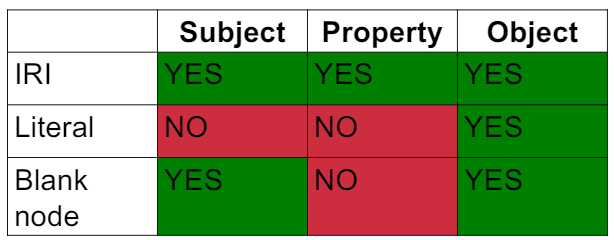
\includegraphics[scale=0.5]{images/3-rdf.PNG}
	\caption{RDF restrictions (in generalized graphs, all is allowed).}
	\label{fig:rdf}
\end{figure}

\paragraph{Syntax}
%TODO (RDF/XML and others)

\paragraph{Querying}
With Cypher (for general) or with SPARQL (for RDF). Cypher does pattern matching to find all subgraphs matching shape of query (also a graph).

%TODO cypher grammar? sparql grammar?


\subsubsection{Neo4j}

\begin{itemize}
    \item Neo4j is an architecture for graph databases. 
    \item No sharding! Graphs are stored as a whole for fast traversal.
    \item Master-slave architecture. Can have multiple master servers = core servers (vs. read replicas = non-core).
    \item Asynchronous (non-blocking) synchronization between master and read replica servers. Allows for reads from all nodes.
    \item Write: either directly to core or do a read replica node sending write also to core. Write is blocked until graph is on absolute majority of every core server (n/2 + 1).
    \item Graphs are stored as graphs in memory (index-free adjacency) but are dissected into their components (nodes, edges, etc.) when stored on disk (fixed-sized records).
\end{itemize}

\paragraph{Storing Stuff}
\begin{itemize}
    \item Label storage: labels of a node are stored as linked list to node.
    \item Property storage: properties of a node are stored as linked list to node where elements are key/value pairs.
    \item Relationship storage: linked list of outgoing edges %TODO something something video
\end{itemize}


%but schema for semantics (not in terms of shape)

\subsubsection{GDB Reading Assignment}

See reading assignment "Graph Databases".

%TODO?







\subsection{Cubes}

\paragraph{Data Warehouse}
Subject-oriented (customers, sales, products, events), integrated (data comes from many applications and ETLed into the data warehouse), time-variant, nonvolatile (load and access, no updates) collection of data in support of management's decision-making process (analyze, report, mine).

%TODO more on ETL?

\paragraph{OLTP vs. OLAP}
See Figure \ref{fig:ovso}.

\begin{figure}[h]
	\centering
	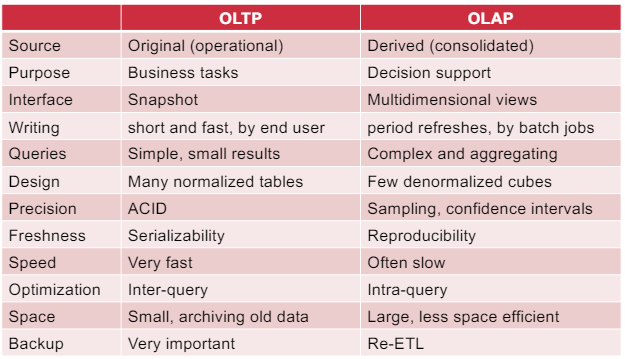
\includegraphics[scale=0.7]{images/3-ovso.PNG}
	\caption{OLTP vs. OLAP.}
	\label{fig:ovso}
\end{figure}

\paragraph{Cube Data Model}
Data (= facts) is stored in multidimensional hypercubes. E.g. year - country - product = key with some value (price or something) - can be empty.

Transform into a table by mapping dimensions into their own fields with cube content as additional field in corresponding row.

\paragraph{Aggregation}
Remove one dimension of the cube.

\paragraph{Slicing}
Extract one stage of cube (for a specific year, give me all countries and products).

\paragraph{Dicing}
Extract sub-cube.

\paragraph{Pivoting}
Turn cube around.

\paragraph{Drill Down}
Zoom in into one dimension while still keeping cube shape.

\paragraph{Drill Up / Roll Up}
In contrast to drill down (e.g. month to year).


\paragraph{Implemenation}
ROLAP - simply as table either with one value per multi-dimensional key or multiple measures (sub-values) - see star / snowflake schemas) - just use SQL here. Or MOLAP with MDX ....... %TODO??






\subsection{Dremel}

See reading assignment "Dremel: Interactive Analysis of Web-Scale Datasets". The following is a brief summary of that paper.

\paragraph{Introduction}
\begin{itemize}
    \item \textbf{Dremel is a scalable, interactive ad hoc query system for analysis of read-only nested data.}
    \item Combine multilevel execution trees and columnar data layout - aggregation queries over huge amounts of rows in seconds.
    \item Shared clusters with commodity hardware.
    \item Dremel can execute many queries usually requiring a sequence of MapReduce jobs but at a fraction of execution time.
    \item Not a replacement for MR, often used in conjunction.
    \item Serving tree and high level language to execute queries natively (no translation to MR jobs).
    \item Column-striped storage representation for nested data (see Figure \ref{fig:dremel}).
    \item Used on top of GFS (distributed storage layer, data is replicated, etc.). (Dremel is like Hive in Hadoop).
\end{itemize}

\begin{figure}[h]
	\centering
	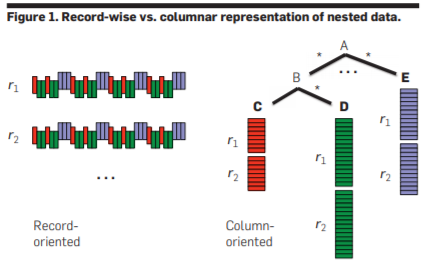
\includegraphics[scale=0.7]{images/3-dremel.PNG}
	\caption{Access A.B.C without anything else.}
	\label{fig:dremel}
\end{figure}

\paragraph{Data Model}


\paragraph{Nested Columnar Store}

\paragraph{Query Language}

\paragraph{Query Execution}

\paragraph{Observations}



